\frame{
	\frametitle{1G: Germany}
	
	\begin{columns}
		\begin{column}{0.4\textwidth}
			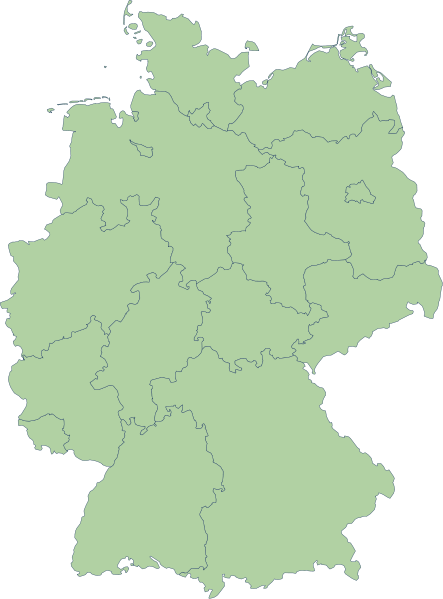
\includegraphics[width=\textwidth]{pictures/deutschland}
		\end{column}
	
		\hfill
	
		\begin{column}{0.59\textwidth}
			\begin{center}
				
\includegraphics[width=0.5\textwidth]{pictures/bundespost}
			\end{center}
			\begin{itemize}
				\item Responsible provider: Deutsche Bundespost
				\item Monopoly of DBP as only provider
				\item Network was finished in 1985, years after Japan, US and NMT
			\end{itemize}
		\end{column}
	\end{columns}
}

\frame{
	\frametitle{1G: Germany}
	
	\begin{columns}
		\begin{column}{0.7\textwidth}
			
\includegraphics[width=0.5\textwidth]{pictures/siemens}
	
			\textbf{Development of the} 
\includegraphics[height=0.3cm]{pictures/cnetz_orig} \textbf{-Net}
	
			\begin{itemize}
				\item Innovation process started in 1979
				\item Siemens was assigned to develop the technology
				\item Intention of creating a superior technology
				\item Start was postponed in favor of advanced technology
				\item Result: The German 1G approach was late
			\end{itemize}
			
		\end{column}
		\hfill
		\begin{column}{0.29\textwidth}
			\begin{figure}[t]
				
\includegraphics[width=\textwidth]{pictures/antenne}
			\end{figure}
		\end{column}
	\end{columns}
}

\frame{
	\frametitle{1G: Germany}
	
	\textbf{Failure factors of the C-Net - Part 1}
	
	\begin{itemize}
		\item \textbf{It was proprietary, a closed system}
			\begin{itemize}
				\item The closed system caused a monopoly for infrastructure and handsets
			\end{itemize}
		\item \textbf{It was expensive}
			\begin{itemize}
				\item Lack of competition in Germany
				\item This also prevented prices from falling
				\item If amount of users reaches capacity limits, prices were raised
				\item In contrast: NMT fixed their technology to cope the demand
			\end{itemize}
	\end{itemize}
}

\frame{
	\frametitle{1G: Germany}
	
	\textbf{Failure factors of the C-Net - Part 2}
	
	\begin{itemize}
		\item \textbf{Only few attracted users}
			\begin{itemize}
				\item Number of subscribers\cite{FuMe2001}:
				\begin{itemize}
					\item C-Net: 17.000
					\item TACS (UK): 122.000
					\item NMT: 330.000 
				\end{itemize}
				\item Missing positive externalities
			\end{itemize}
		\item \textbf{The lack of leadership}
			 \begin{itemize}
				 \item Neither government nor companies formed a committee
			 \end{itemize}
	\end{itemize}
}